\documentclass[10pt]{article}
% Shared preamble for margin-stack prototypes.
% Mirrors the production geometry: 2.6cm-wide rungs, optional 0.3cm spine at
% x=2.85-3.15, \rmfamily labels (Palatino under the real build).
\usepackage{tikz}
\usetikzlibrary{positioning,calc,patterns,decorations.pathmorphing,decorations.pathreplacing}
\usepackage{xcolor}
\usepackage[paperwidth=20cm,paperheight=25cm,margin=8mm]{geometry}
\pagestyle{empty}

% Volume accents (from books/shared/tex/theme-colors-vol*.tex)
\definecolor{crimson}{HTML}{A51C30}      % vol1  Harvard Crimson
\definecolor{ethzblue}{HTML}{1F407A}     % vol2  ETH Zurich Blue
\definecolor{amethyst}{HTML}{581C87}     % vol3  Amethyst
\definecolor{emeraldpine}{HTML}{1A4D3E}  % vol4  Emerald Pine

% One rung. #1 y-bottom  #2 height  #3 label  #4 intensity 0-100  #5 accent
\newcommand{\protorung}[5]{%
  \ifnum#4=0
    \def\fillcol{black!5}\def\textcol{black!30}%
  \else
    \def\fillcol{#5!#4!white}%
    \ifnum#4>50 \def\textcol{white}\else \def\textcol{#5}\fi
  \fi
  \node[draw=white,line width=0.5pt,fill=\fillcol,minimum width=2.6cm,
        minimum height=#2 cm,anchor=south west,inner sep=0pt] (b) at (0,#1) {};
  \node[anchor=west,text=\textcol,font=\rmfamily\scriptsize\bfseries]
        at ($(b.west)+(0.12,0)$) {#3};
}

% Rung with a right-aligned secondary label (cadence, rate, count).
% #1 y  #2 h  #3 label  #4 right-label  #5 intensity  #6 accent
\newcommand{\protorungrt}[6]{%
  \ifnum#5=0
    \def\fillcol{black!5}\def\textcol{black!30}%
  \else
    \def\fillcol{#6!#5!white}%
    \ifnum#5>50 \def\textcol{white}\else \def\textcol{#6}\fi
  \fi
  \node[draw=white,line width=0.5pt,fill=\fillcol,minimum width=2.6cm,
        minimum height=#2 cm,anchor=south west,inner sep=0pt] (b) at (0,#1) {};
  \node[anchor=west,text=\textcol,font=\rmfamily\scriptsize\bfseries]
        at ($(b.west)+(0.12,0.09)$) {#3};
  \node[anchor=west,text=\textcol,font=\rmfamily\fontsize{4.6}{5}\selectfont,opacity=0.85]
        at ($(b.west)+(0.12,-0.12)$) {#4};
}

% Vertical cross-cutting spine at x=2.85..3.15 (vol1 data bar / vol3 trajectory).
% #1 y-bottom  #2 y-top  #3 word  #4 intensity  #5 accent
\newcommand{\protospine}[5]{%
  \fill[#5!#4!white,rounded corners=1.5pt] (2.85,#1) rectangle (3.15,#2);
  \pgfmathsetmacro{\midy}{(#1+#2)/2}
  \ifnum#4>50 \def\spinecol{white}\else \def\spinecol{#5}\fi
  \node[rotate=90,text=\spinecol,font=\rmfamily\fontsize{5}{6}\selectfont\bfseries]
        at (3.0,\midy) {#3};
}

% Caption under a prototype.
\newcommand{\protocap}[2]{%
  \begin{minipage}[t]{3.0cm}\raggedright
  \textbf{\footnotesize #1}\\[1pt]{\fontsize{6.5}{8}\selectfont #2}
  \end{minipage}}

% vol3-scale rung: 4.8pt label, matching tex/agent-stack-vol3.tex exactly.
\newcommand{\protorungsm}[5]{%
  \ifnum#4=0 \def\fillcol{black!5}\def\textcol{black!30}%
  \else \def\fillcol{#5!#4!white}%
    \ifnum#4>50 \def\textcol{white}\else \def\textcol{#5}\fi \fi
  \node[draw=white,line width=0.4pt,fill=\fillcol,minimum width=2.6cm,
        minimum height=#2 cm,anchor=south west,inner sep=0pt] (b) at (0,#1) {};
  \node[anchor=west,text=\textcol,font=\rmfamily\fontsize{4.8}{5.2}\selectfont\bfseries]
        at ($(b.west)+(0.12,0)$) {#3};
}
\newcommand{\protorungsmrt}[6]{%
  \ifnum#5=0 \def\fillcol{black!5}\def\textcol{black!30}%
  \else \def\fillcol{#6!#5!white}%
    \ifnum#5>50 \def\textcol{white}\else \def\textcol{#6}\fi \fi
  \node[draw=white,line width=0.4pt,fill=\fillcol,minimum width=2.6cm,
        minimum height=#2 cm,anchor=south west,inner sep=0pt] (b) at (0,#1) {};
  \node[anchor=west,text=\textcol,font=\rmfamily\fontsize{4.8}{5.2}\selectfont\bfseries]
        at ($(b.west)+(0.12,0.07)$) {#3};
  \node[anchor=west,text=\textcol,font=\rmfamily\fontsize{3.9}{4.4}\selectfont,opacity=0.85]
        at ($(b.west)+(0.12,-0.09)$) {#4};
}

\begin{document}
\noindent{\Large\bfseries The series bracket --- image 4's device, applied to four volumes}\\[2pt]
{\footnotesize The classic architecture ladder's real contribution is not its layer list but the
left-hand bracket that says \emph{this book owns these levels}. Two candidate spines below.
The second is the honest one.}\\[7mm]

\noindent
% ---------- CANDIDATE 1: the naive stacked spine ----------
\begin{minipage}[t]{7.4cm}
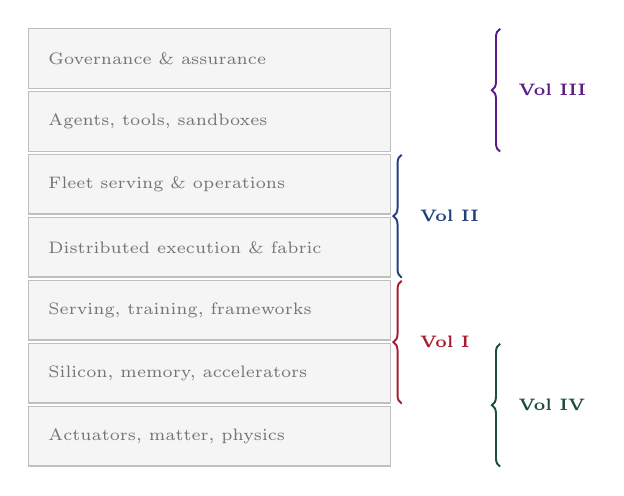
\begin{tikzpicture}[x=1cm,y=1cm]
  \foreach \y/\lbl in {
    5.0/{Governance \& assurance},
    4.2/{Agents, tools, sandboxes},
    3.4/{Fleet serving \& operations},
    2.6/{Distributed execution \& fabric},
    1.8/{Serving, training, frameworks},
    1.0/{Silicon, memory, accelerators},
    0.2/{Actuators, matter, physics}} {
    \node[draw=black!25,line width=0.4pt,fill=black!4,minimum width=4.6cm,
          minimum height=0.76cm,anchor=south west,inner sep=0pt] at (0,\y) {};
    \node[anchor=west,font=\rmfamily\fontsize{6.5}{7.5}\selectfont,text=black!55]
          at (0.14,\y+0.38) {\lbl};
  }
  \draw[decorate,decoration={brace,amplitude=3pt},crimson,line width=0.7pt]
        (4.75,1.0) -- (4.75,2.56) node[midway,right=3pt,text=crimson,
        font=\rmfamily\fontsize{6}{7}\selectfont\bfseries] {Vol I};
  \draw[decorate,decoration={brace,amplitude=3pt},ethzblue,line width=0.7pt]
        (4.75,2.6) -- (4.75,4.16) node[midway,right=3pt,text=ethzblue,
        font=\rmfamily\fontsize{6}{7}\selectfont\bfseries] {Vol II};
  \draw[decorate,decoration={brace,amplitude=3pt},amethyst,line width=0.7pt]
        (6.0,4.2) -- (6.0,5.76) node[midway,right=3pt,text=amethyst,
        font=\rmfamily\fontsize{6}{7}\selectfont\bfseries] {Vol III};
  \draw[decorate,decoration={brace,amplitude=3pt},emeraldpine,line width=0.7pt]
        (6.0,0.2) -- (6.0,1.76) node[midway,right=3pt,text=emeraldpine,
        font=\rmfamily\fontsize{6}{7}\selectfont\bfseries] {Vol IV};
\end{tikzpicture}\\[4mm]
\textbf{\footnotesize Candidate 1 --- one ladder, four brackets}\\[1pt]
{\fontsize{7}{9}\selectfont\raggedright
This is the literal port of image~4, and it does not survive contact. The brackets have to
jump the ladder and overlap: vol4 owns the bottom \emph{and} reaches up into governance,
vol3 sits on top of vol2's serving layer rather than beside it, and governance belongs to
three volumes at once. The four stacks are not four bands of one ladder.\par}
\end{minipage}\hfill
% ---------- CANDIDATE 2: the blast-radius spine ----------
\begin{minipage}[t]{8.6cm}
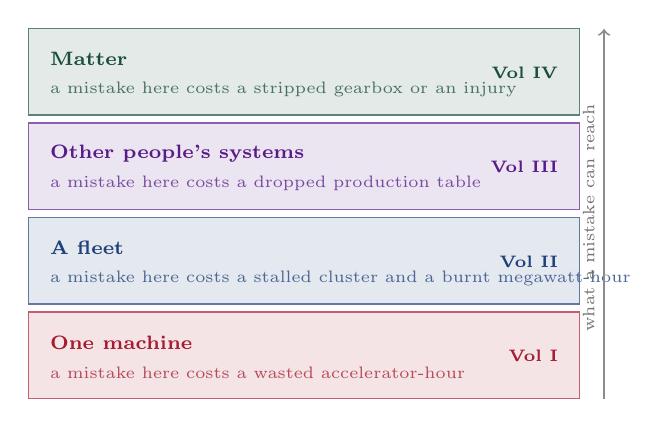
\begin{tikzpicture}[x=1cm,y=1cm]
  \foreach \y/\c/\v/\lbl/\dmg in {
    0.2/crimson/{Vol I}/{One machine}/{a wasted accelerator-hour},
    1.4/ethzblue/{Vol II}/{A fleet}/{a stalled cluster and a burnt megawatt-hour},
    2.6/amethyst/{Vol III}/{Other people's systems}/{a dropped production table},
    3.8/emeraldpine/{Vol IV}/{Matter}/{a stripped gearbox or an injury}} {
    \node[draw=\c!70,line width=0.5pt,fill=\c!12,minimum width=7.0cm,
          minimum height=1.10cm,anchor=south west,inner sep=0pt] at (0,\y) {};
    \node[anchor=west,font=\rmfamily\fontsize{7}{8}\selectfont\bfseries,text=\c]
          at (0.16,\y+0.72) {\lbl};
    \node[anchor=west,font=\rmfamily\fontsize{5.8}{7}\selectfont,text=\c!80]
          at (0.16,\y+0.34) {a mistake here costs \dmg};
    \node[anchor=east,font=\rmfamily\fontsize{6}{7}\selectfont\bfseries,text=\c]
          at (6.86,\y+0.55) {\v};
  }
  \draw[->,black!45,line width=0.7pt] (7.32,0.2) -- (7.32,4.9);
  \node[rotate=90,anchor=south,font=\rmfamily\fontsize{6}{7}\selectfont,text=black!55]
        at (7.32,2.5) {what a mistake can reach};
\end{tikzpicture}\\[4mm]
\textbf{\footnotesize Candidate 2 --- one axis: blast radius}\\[1pt]
{\fontsize{7}{9}\selectfont\raggedright
The four volumes do differ along one real axis, and it is the book's own argument: what a
mistake is allowed to damage. Each volume takes the previous one's constraints and adds a
consequence that cannot be rolled back. This nests cleanly, needs no overlapping brackets,
and tells a reader holding all four why there are four.\par}
\end{minipage}
\end{document}
